% Created 2024-02-27 Tue 14:22
% Intended LaTeX compiler: pdflatex
\documentclass[presentation]{beamer}
\usepackage[utf8]{inputenc}
\usepackage[T1]{fontenc}
\usepackage{graphicx}
\usepackage{longtable}
\usepackage{wrapfig}
\usepackage{rotating}
\usepackage[normalem]{ulem}
\usepackage{amsmath}
\usepackage{amssymb}
\usepackage{capt-of}
\usepackage{hyperref}
\mode<beamer>{\usetheme{Madrid}}
\definecolor{SUred}{rgb}{0.59375, 0, 0.17969} % SU red (primary)
\definecolor{SUblue}{rgb}{0, 0.17578, 0.38281} % SU blue (secondary)
\setbeamercolor{palette primary}{bg=SUred,fg=white}
\setbeamercolor{palette secondary}{bg=SUblue,fg=white}
\setbeamercolor{palette tertiary}{bg=SUblue,fg=white}
\setbeamercolor{palette quaternary}{bg=SUblue,fg=white}
\setbeamercolor{structure}{fg=SUblue} % itemize, enumerate, etc
\setbeamercolor{section in toc}{fg=SUblue} % TOC sections
% Override palette coloring with secondary
\setbeamercolor{subsection in head/foot}{bg=SUblue,fg=white}
\setbeamercolor{date in head/foot}{bg=SUblue,fg=white}
\institute[SU]{Shenandoah University}
\titlegraphic{
\includegraphics[width=0.5\textwidth]{\string~/Documents/suLogo/suLogo.pdf}}
\newcommand{\R}{\mathbb{R}}
\usepackage{tikz}
\usepackage{pgfplots}
\usetheme{default}
\author{Chase Mathison\thanks{cmathiso@su.edu}}
\date{28 February 2024}
\title{Trig Substitution, Part II}
\hypersetup{
 pdfauthor={Chase Mathison},
 pdftitle={Trig Substitution, Part II},
 pdfkeywords={},
 pdfsubject={},
 pdfcreator={Emacs 29.1 (Org mode 9.6.7)}, 
 pdflang={English}}
\begin{document}

\maketitle

\section{Announcements}
\label{sec:org9f80f9f}
\begin{frame}[label={sec:orgd6e27f8}]{Announcements}
\begin{enumerate}
\item Homework
\item Office hours, 10am - 11am
\end{enumerate}
\end{frame}

\begin{frame}[label={sec:orgeb97ebd}]{Integrals involving \(\sqrt{x^2-a^2}\)}
It should be no surprise that we can integrate functions of the form
\(\sqrt{x^2-a^2}\) as well:

\begin{center}
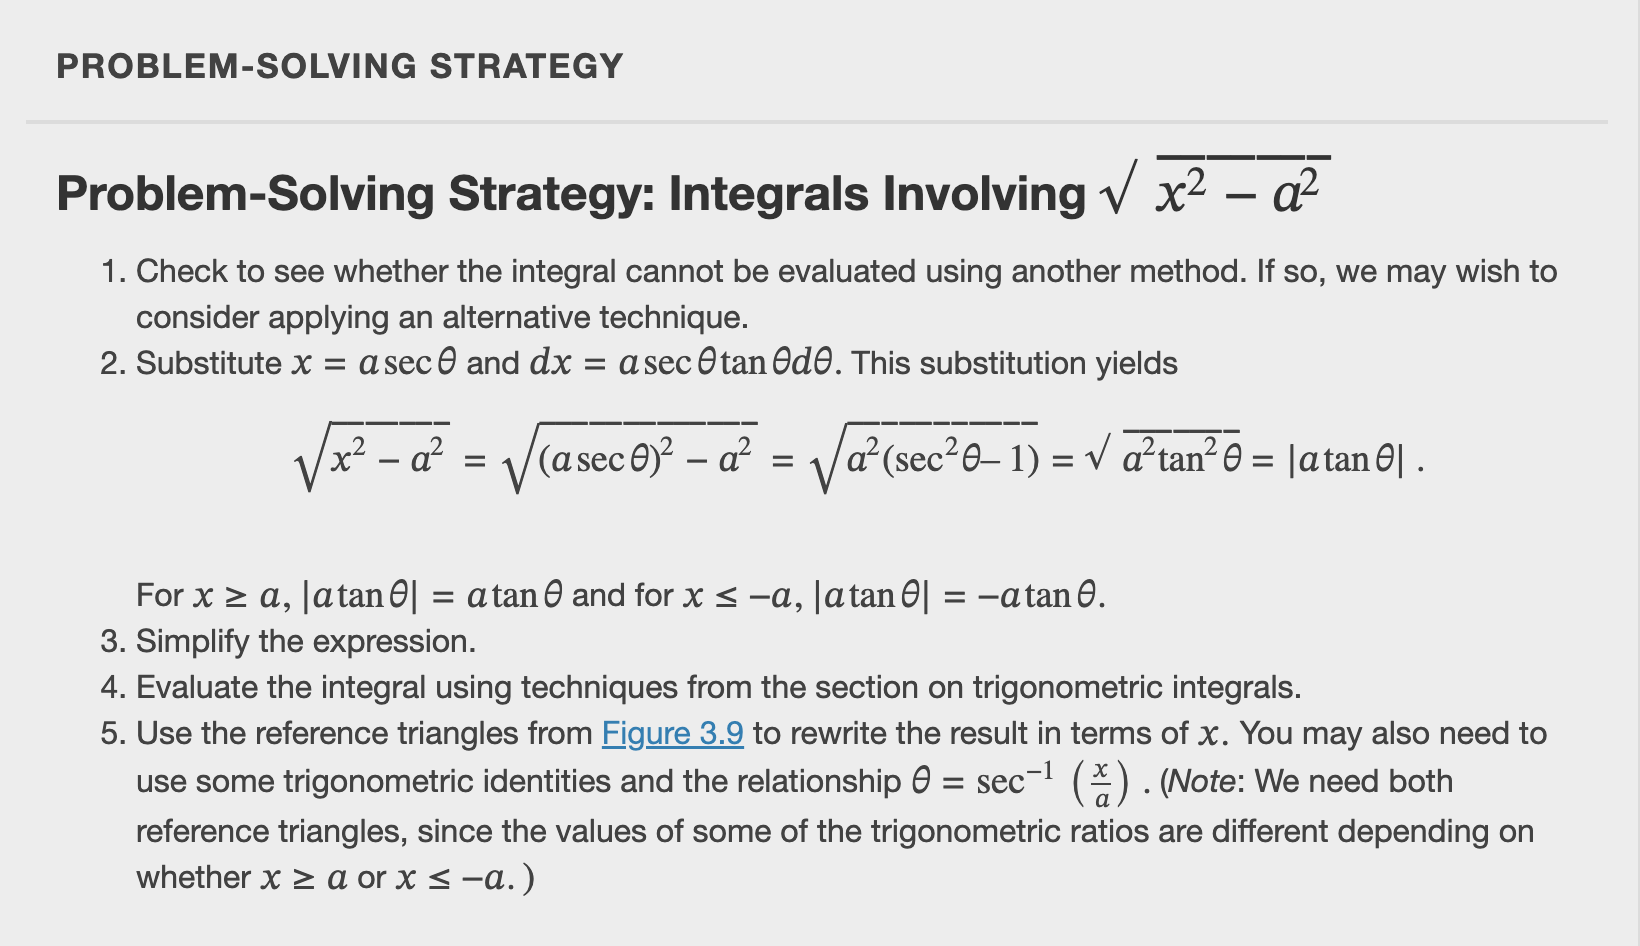
\includegraphics[width=0.8\textwidth]{../img/trigSub3.png}
\end{center}
\end{frame}

\begin{frame}[label={sec:org3c35d60}]{Example}
Evaluate
\[
\int\limits_{}^{} \sqrt{2x^2 - 8}\,dx \]
\vspace{10in}
\end{frame}

\begin{frame}[label={sec:org253d8da}]{Example}
\end{frame}

\begin{frame}[label={sec:org528cd15}]{Example}
Find
\[\int\limits_2^3 \sqrt{2x^2-8}\,dx \]
\vspace{10in}
\end{frame}


\begin{frame}[label={sec:org24c84a5}]{Completing the square}
Before we look at the next example, we need to discuss how to
\emph{complete the square}. (Something that technically is supposed to be
taught in precalc, but hardly ever is).

We would like to rewrite
\[ax^2 + bx + c \]
in the form
\[ a\left( x-h \right)^2 + k. \]

Let's figure out what \(h\) and \(k\) need to be.
\vspace{10in}
\end{frame}

\begin{frame}[label={sec:org04a28e6}]{Completing the square}
\end{frame}

\begin{frame}[label={sec:org5d35e0d}]{Completing the square}
Find
\[
\int\limits_{}^{} \frac{2}{\sqrt{x^2+2x}}dx \]
\vspace{10in}
\end{frame}

\begin{frame}[label={sec:org392d168}]{Completing the square}
\end{frame}

\begin{frame}[label={sec:org3ffc0a0}]{Examples}
Evaluate
\[
\int\limits_{}^{}\frac{dx}{\sqrt{1+9x^2}} \]
\vspace{10in}
\end{frame}

\begin{frame}[label={sec:org98b940a}]{Examples}
\end{frame}
\end{document}